%
% template.tex -- slide template
%
% (c) 2021 Prof Dr Andreas Müller, OST Ostschweizer Fachhochschule
%
\bgroup
\begin{frame}
\setlength{\abovedisplayskip}{5pt}
\setlength{\belowdisplayskip}{5pt}
\frametitle{Kugeldreiecke}
\begin{center}
\begin{tikzpicture}[>=latex,thick]
\uncover<1>{
\node at (0,0) {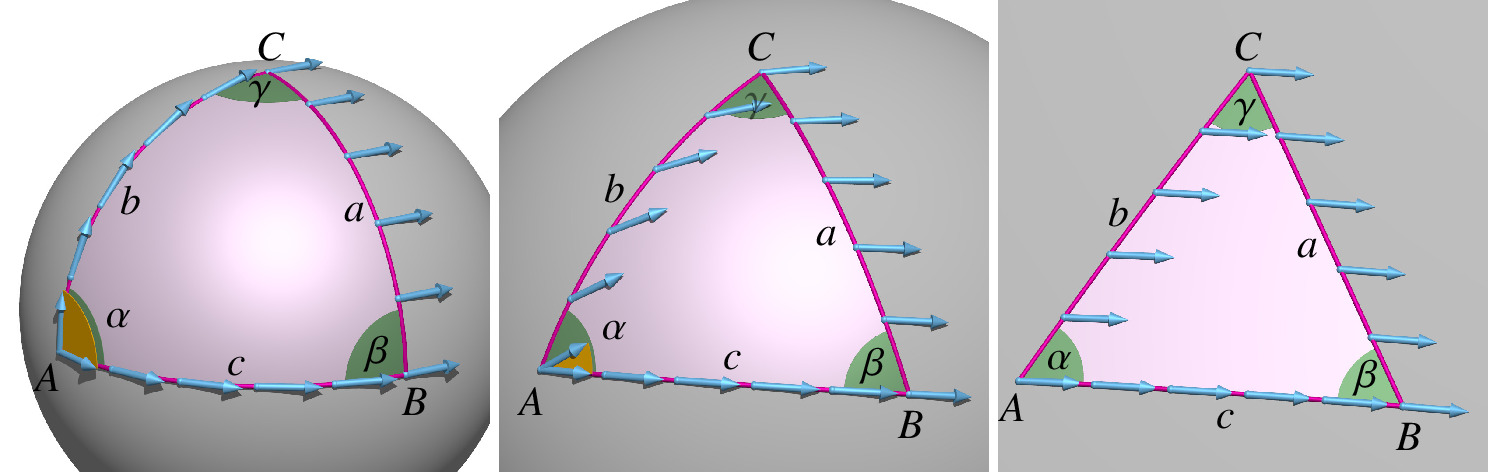
\includegraphics[width=13.0cm]{../../buch/chapters/110-kruemmung/images/exzess-notes.jpg}};
}
\uncover<2>{
\node at (0,0) {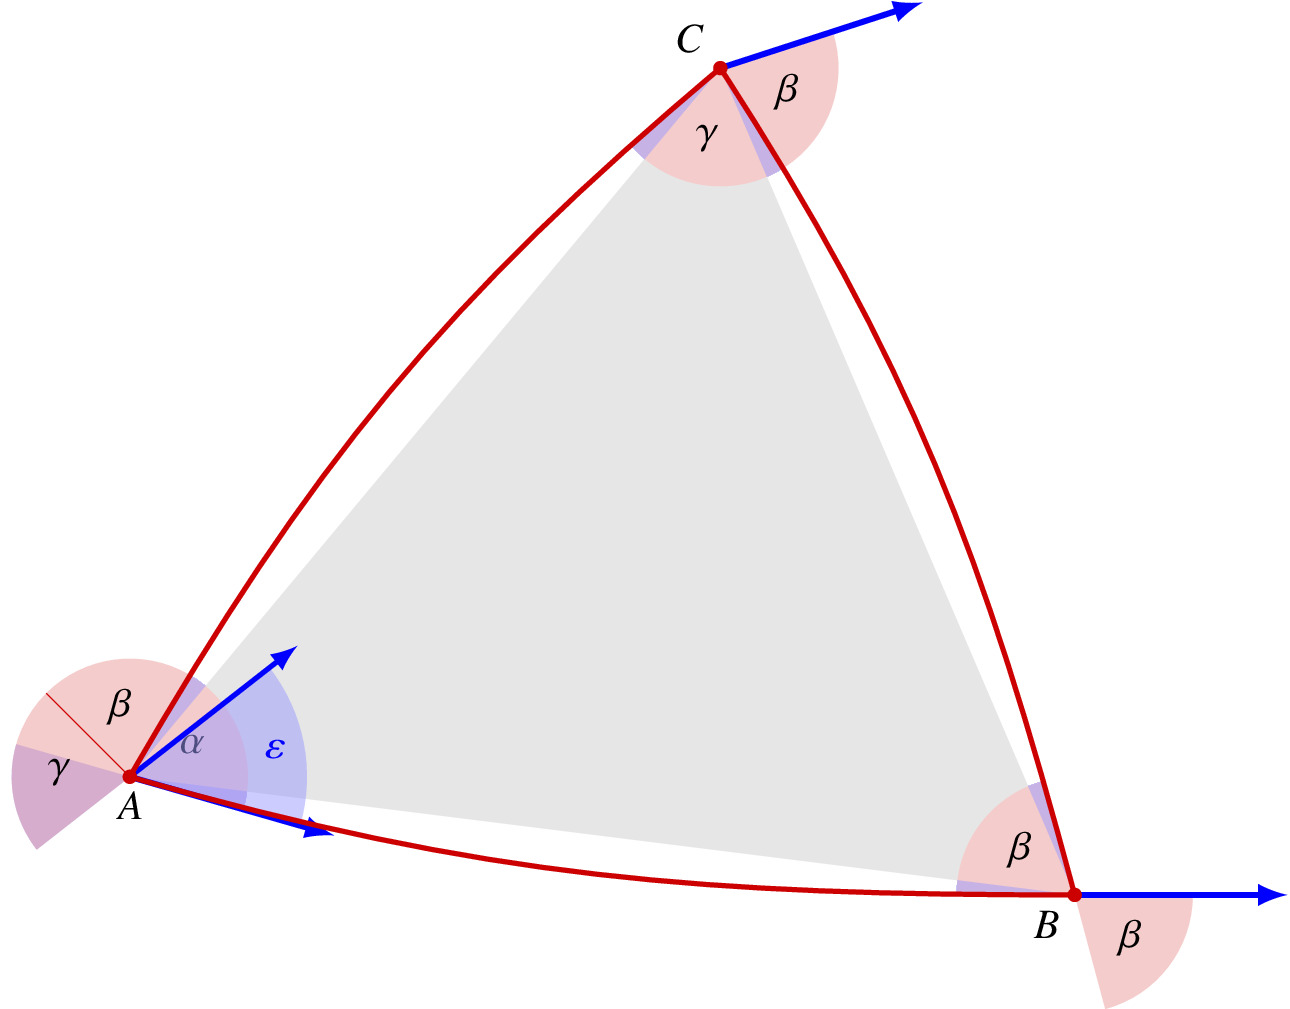
\includegraphics[width=10.0cm]{../../buch/chapters/110-kruemmung/images/drehung-notes.jpg}};
}
\end{tikzpicture}
\end{center}
\end{frame}
\egroup
